\section{Résultats}

\paragraph*{Pouvoirs calorifiques théoriques}
A l'aide des équations chimiques de combustion des 4 combustibles utilisés, présentées dans les \autoref{eq:ethanol_combustion}, \autoref{eq:methanol_combustion}, \autoref{eq:butane_combustion} et \autoref{eq:propane_combustion}, et en utilisant celles-ci avec l'\autoref{eq:chaleur_réaction} il est possible de déterminer le pouvoir calorifique théorique des espèces utilisées. Les chaleurs de formation des espèces chimiques et les masses molaires nécessaires à ce calcul sont données dans le \autoref{tab:enthalpie_formation}.

\begin{table}[h]
    \centering
    \begin{tabulary}{\linewidth}{C C C}
        \toprule
        Espèce chimique & Enthalpie de formation \(\Delta H\) [\si{\kilo\joule\per\mole}] & Masse molaire \(\rho\) [\si{\gram\per\mole}]\\
        \midrule
        Ethanol & -276 \(\pm\) 2 & 46.1 \(\pm\) 0.1 \\
        Méthanol & -238.4 \(\pm\) 0.5 & 32.0 \(\pm\) 0.1 \\
        Butane & -125.6 \(\pm\) 0.7 & 58.1 \(\pm\) 0.1\\
        Propane & -104.7 \(\pm\) 0.5 & 44.1 \(\pm\) 0.1\\
        \ce{O2} & 0 \(\pm\) 0.1 & / \\
        \ce{CO2} & -393.5 \(\pm\) 0.1 & / \\
        \ce{H2O} & -241.8 \(\pm\) 0.1 & / \\
        \bottomrule
    \end{tabulary}
    \caption{Chaleur de formation de différentes espèces chimiques et masses molaires nécessaires au calcul \cite{notice} \cite{NIST}}
    \label{tab:enthalpie_formation}
\end{table}

Afin d'obtenir le pouvoir calorifique théorique des mélanges éthanol-méthanol et butane-propane il est possible d'effectuer une moyenne pondérée sur les pouvoirs calorifiques obtenus pour chaque espèce. La pondération de cette moyenne est égale aux proportions respectives de chaque composant dans le mélange. Les valeurs obtenues de cette manière sont présentées dans le \autoref{tab:pouvoir_calorifique}.

\paragraph*{Analyse expérimentale de la combustion de l'éthanol-méthanol}
Les valeurs du pouvoir calorifique de la combustion de l'éthanol sont calculées avec l'\autoref{eq:pouvoir_calorifique}. À la fin de toutes les mesures, une masse d'eau de condensation totale \(\Delta M_\textrm{c,tot} = (4.8 \pm 0.1)\) \si{\gram} a été récupérée, donnant une masse \(\Delta M_c = (0.30 \pm 0.01)\) \si{\gram}. La mesure a été effectuée 16 fois et les résultats sont reportés dans la \autoref{fig:H_etanol}. La formule pour le calcul des erreurs est donné dans l'\autoref{sec:erreurs}. La valeur moyenne \(\langle H \rangle\) des mesures est reportée dans le \autoref{tab:pouvoir_calorifique}.

\paragraph*{Analyse expérimentale de la combustion du butane-propane}
En suivant le même procédé, le pouvoir calorifique de la combustion du mélange butane-propane a été déterminée. La masse d'eau condensée totale était \(\Delta M_\textrm{c,tot} = (37.6 \pm 0.1)\) \si{\gram}, donnant alors \(\Delta M_c = (3.13 \pm 0.01)\) \si{\gram} sur chaque mesure. Les résultats des 12 mesures effectuées sont visibles dans la \autoref{fig:H_gaz_camping}. La valeur moyenne \(\langle H \rangle\) des mesures est reportée dans le \autoref{tab:pouvoir_calorifique}.

L'écart relatif entre les valeurs théoriques \(H_\textrm{théo}\) et expérimentales \(H_\textrm{exp}\) sont calculés avec l'\autoref{eq:ecart_rel}

\begin{figure}[h]
    \centering
    \begin{subfigure}{0.5\linewidth}
        \centering
        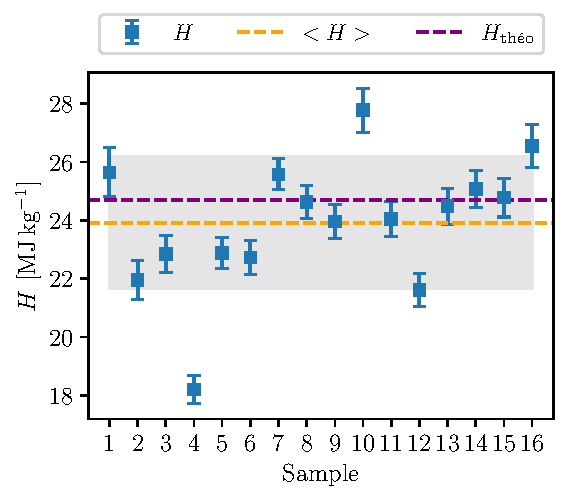
\includegraphics[width=\linewidth]{figures/ethanol.pdf}
        \caption{}
        \label{fig:H_etanol}
    \end{subfigure}%
    \begin{subfigure}{0.5\linewidth}
        \centering
        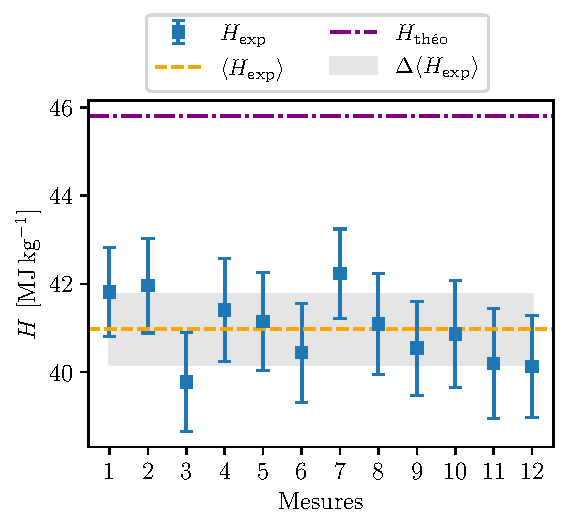
\includegraphics[width=\linewidth]{figures/gaz_camping.pdf}
        \caption{}
        \label{fig:H_gaz_camping}
    \end{subfigure}
    \caption{Pouvoirs calorifiques de combustion calculés pour (a) le mélange éthanol-méthanol (b) le gaz de camping}
\end{figure}

\begin{table}[h]
    \centering
    \begin{tabulary}{\linewidth}{C C C C}
        \toprule
        Combustible & \(H_\textrm{théo}\) [\si{\mega\joule\per\kilo\gram}] & \(\langle H_\textrm{exp} \rangle\) [\si{\mega\joule\per\kilo\gram}] & Écart relatif \(a\) \\
        \midrule
        88\% Éthanol 12\% Méthanol & \(26.0 \pm 0.1\) & \(24 \pm 2\) & \(8.0 \pm 0.6\)\%\\
        80\% Butane 20\% Propane & \(45.8 \pm 0.1\) & \(41 \pm 1\) & \(10.7 \pm 0.6\)\% \\
        \bottomrule
    \end{tabulary}
    \caption{Valeurs théoriques et expérimentales des combustibles}
    \label{tab:pouvoir_calorifique}
\end{table}

\paragraph*{\ce{CO2} produit}
Le \ce{CO2} produit lors de la combustion est donné par l'\autoref{eq:masse_co2}. Puisque le débit était constant, deux mesures avec une masse d'eau \(\Delta M\) donnent un temps de combustion similaire. Pour une masse d'eau \(\Delta M = (910 \pm 2)\) \si{\gram} pour les deux combustibles, la masse de \ce{CO2} libéré est
\begin{align*}
    m_\textrm{CO2,éthanol-méthanol} &= (3.01 \pm 0.06)\ \si{\gram} \\
    m_\textrm{CO2,butane-propane} &= (1.86 \pm 0.05)\ \si{\gram}
\end{align*}
